%%%%%%%%%%%%%%%%%%%%%%%%%%%%%%%%%%%%%%%%%%%%%%%%%%%%%%%%%%%%%%%%%%%%%%%%%%%%%%%%
%2345678901234567890123456789012345678901234567890123456789012345678901234567890
%        1         2         3         4         5         6         7         8


%\documentclass[twocolumn,journal]{IEEEtran}
\documentclass[twocolumn,journal]{IEEEtran}
%\documentclass[letterpaper, 10 pt, conference]{ieeeconf}  % Comment t                                                      his line out
                                                          % if you need a4paper
%\documentclass[a4paper, 10pt, conference]{ieeeconf}      % Use this line for a4
                                                          % paper

\IEEEoverridecommandlockouts                           % This command is only
                                                          % needed if you want to
                                                          % use the \thanks command
\overrideIEEEmargins
% See the \addtolength command later in the file to balance the column lengths
% on the last page of the document

\newtheorem{theorem}{Theorem}
\newtheorem{definition}{Definition}
\newtheorem{corollary}{Corollary}
\newtheorem{example}{Example}
\newtheorem{assumption}{Assumption}
\newtheorem{hypothesis}{Hypothesis}
\newtheorem{lemma}{Lemma}
\newtheorem{remark}{Remark}
\newtheorem{notation}{Notation}
\newtheorem{algorithm}{Algorithm}
\newtheorem{property}{Property}
%\newcommand{\for}{\textbf{for}}
%\newcommand{\STATE}{\quad}
% The following packages can be found on http:\\www.ctan.org
\usepackage{graphicx}
\usepackage{subfig}% for pdf, bitmapped graphics files
%\usepackage{epsfig} % for postscript graphics files
\usepackage{mathptmx} % assumes new font selection scheme installed
\usepackage{times} % assumes new font selection scheme installed
\usepackage{amsmath} % assumes amsmath package installed
\usepackage{amssymb}  % assumes amsmath package installed
\usepackage{algorithm}
\usepackage{algorithmic}
\usepackage{multirow}
\usepackage{amsmath}
\usepackage{xcolor}

\title{\LARGE \bf
Stability of (n,k) Nonlinear feedback shift registers}

\author{Meilin Li, Jianquan Lu, Tingwen Huang, Jinde Cao \IEEEmembership{Fellow,~IEEE}
\thanks{This work was supported by the National Natural Science Foundation of China under Grant No. 61573102, and China Postdoctoral Science Foundation under Grant No. 2014M560377 and 2015T80483, and Jiangsu Province Six Talent Peaks Project under Grant 2015-ZNDW-002. }%
\thanks{Meilin Li is is with the Department of Mathematics, Southeast
University, Nanjing 210096, China {\tt\small 220151318@seu.edu.cn}}
\thanks{ Jianquan Lu is with the Department of Mathematics, Southeast
University, Nanjing 210096, China, and also with the Potsdam
Institute for Climate Impact Research, Telegraphenberg, D-14415
Potsdam, Germany
{\tt\small jqluma@seu.edu.cn;jqluma@gmail.com}}
\thanks{Tingwen Huang is with Texas AM University at Qatar, Dc/o Qatar Foundation, PO Box 5825, Doha, Qatar}
\thanks{ Jinde Cao is
with the Department of Mathematics, Southeast University, Nanjing
210096, China {\tt\small jdcao@seu.edu.cn}}
\thanks{}
\thanks{}
\thanks{} }
\begin{document}

\maketitle
\thispagestyle{empty}
\pagestyle{empty}

%%%%%%%%%%%%%%%%%%%%%%%%%%%%%%%%%%%%%%%%%%%%%%%%%%%%%%%%%%%%%%%%%%%%%%%%%%%%%%%%
\begin{abstract}
In this paper, the $(n,k)$ nonlinear feedback shift registers (NFSRs) are regarded as a Boolean network (BN). Semi-tensor product (STP) of matrices is used to convert $(n,k)$ NFSRs into an equivalent algebraic equation. Based on STP of matrices, a novel way is proposed to study stability of $(n,k)$ NFSRs and the period of $(n,k)$ NFSRs. Firstly,
\end{abstract}

\begin{keywords}
$(n,k)$ NFSRs, stability, semi-tensor product, Boolean network
\end{keywords}

\section{introduction}
Information security is very important for our society. There are many confidential information about financial status, research, products for different organizations. In order to protect the confidential information from leakage, the stream cipher has been widely used in encryption. The main building blocks of stream cipher is nonlinear shift registers (NFSR). NFSR can produce pseudo-random sequences.

There are two types of NFSR: (1) Fibonacci NFSR; (2) Galois NFSR. Fibonacci NFSR is shown in Fig.\ref{fsr}. Fibonacci NFSR consists $n$ binary storage elements from left to right as $n-1,n-2,...,1,0$. Every $i$-th $0\leq i\leq n-2$ bit is update their values by the value of $(i+1)$-th bit, and the value of $(n-1)$-th bit is updated by feedback function $f$ depending on values of bits of $0,1,...,n-1$.While the Galois NFSR shown in Fig.\ref{gsr} is different from Fibonacci NFSR. In Galois NFSR, the value of every bit is updated by  it's own feedback function which at most relate to every bit.

In order to improve the speed of output sequence generation, E. Dubrova proposed a new type of NFSR named $(n,k)$ NFSR in \cite{Dubrova2008On}. An $(n,k)$ NFSR can be considered as a generalization of the Galois NFSR. In an $(n,k)$ NFSR, every bit is updated by a feedback function, which is a nonlinear function relating to value of $(i+1)mod~n$-th bit and up to values of $k-1$ other bits.

\begin{figure}
\centering
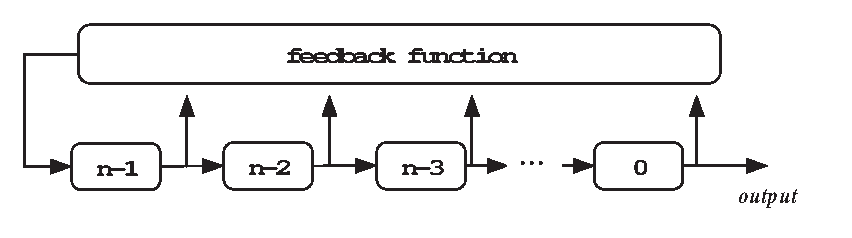
\includegraphics[width=3in]{fsr.eps}
\caption{The Fibonacci NLFSR}
\label{fsr}
\end{figure}
\begin{figure}
\centering
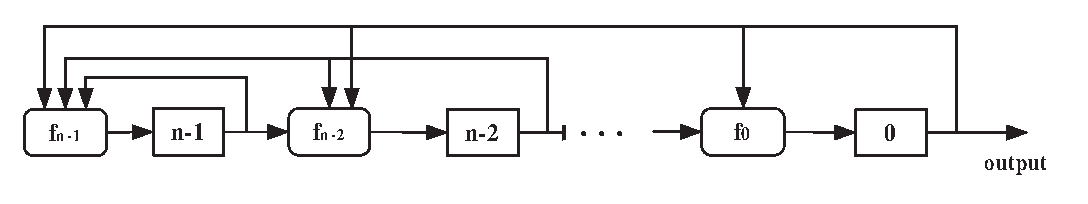
\includegraphics[width=3in]{Galois.eps}
\caption{The Fibonacci NLFSRs}
\label{gsr}
\end{figure}

\section{preliminaries}
In this section, we first review the STP of matrices briefly. Then the multi-linear
form of nonlinear Boolean function that is obtained by using the semi-tensor product is recalled. Finally, we regard $(n,k)$ NFSRs as a BN. Based on STP, $(n,k)$ NFSRs are converted into a multi-linear forms. We first give some notations used in this paper.
\begin{itemize}
  \item $\mathcal{D}=\{0,1\}$.
  \item $I_n:$ the identity matrix of dimension $n$.
  \item $\delta^i_{2^n}:$ the $i$-th column of identity matrix $I_n$.
  \item $\Delta_{2^n}=\{\delta^i_{2^n}|i=1,2,3,...,2^n\}$.
  \item $\mathcal{L}_{n\times m}:$ the set of $n\times m$ matrices, whose column belong to $\Delta_{n}$. For a matrix $L\in\mathcal(L)_{n\times m}$, and $L=[\delta^{i_1}_{n}~ \delta^{i_2}_{n}~ ... ~ \delta^{i_m}_{n}]$, we write $L=\delta_{2^n}[i_1~ i_2~ ... ~ i_m]$ for simplicity. \item $col_i(L):$ the $i$-th column of matrix $L$.
  \item $col(L):$ the set of all column of matrix $L$.
  \item $\mathbb{R}:$ the set of all real number.
  \item $N:$ the set of all integers.
\end{itemize}


\subsection{Semi-tensor product of matrices}
In this subsection, the definition of STP is given. The the multi-linear form of nonlinear Boolean function is obtained by using the semi-tensor product.

\begin{definition}\cite{Cheng2011Analysis}
Let $A\in\mathbb{R}^{n\times m}$, $B\in \mathbb{R}^{p\times q}$. The \textit{semi-tensor product} of $A$ and $B$ is defined as:
\begin{equation}
A\ltimes B=(A\otimes I_{\frac{l}{m})}(B\otimes I_{\frac{l}{p}})
\end{equation}
where $l$ is the least common multiple of $m$ and $p$.
\end{definition}

Obviously, if $m=p$ in Definition \ref{stp}, then the STP of $A$ and $B$ is reduced to their conventional matrix product $AB$.

We identify $\Delta_{2}\sim \mathcal{D}$ i.e $(\delta^1_2\sim 1,\delta^2_2\sim 0)$, and $\delta^1_2(\delta^2_2)$ is called the vector form of logical value $1(0)$.

\begin{lemma}\label{lemma1}\cite{Cheng2011Analysis}
Any Boolean function $f(x_1,x_2,...,x_n)$ with variables $x_1,x_2,...,x_n\in \Delta_2$ can be expressed as a multi-linear form:
\begin{equation}
f(x_1,x_2,...,x_n)=Fx_1\ltimes x_2\ltimes ...\ltimes x_n.
\end{equation}
where $F\in \mathcal{L}_{2\times 2^n}$ is called the \textit{structure matrix} of $f$, and $F$ can be uniquely expressed as
\begin{equation}
F=\left[
    \begin{array}{cccc}
      s_1 & s_2 & ... & s_{2^{n}} \\
      1-s_1 & 1-s_2 & ... & 1-s_{2^n} \\
    \end{array}
  \right]
\end{equation}
with $[s_1,s_2,...,s_{2^n}]$ being the truth table of $f$, arranged in the reverse alphabet order.
\end{lemma}

In the following, we omit the symbol $\ltimes$ for simplicity.


\subsection{$(n,k)$ NFSRs}
A $(n,k)$ NFSRs consist of $n$ binary memory device called bits. The output of a $(n,k)$ NFSRs is the value of the $0$-th bit. A $(n,k)$ NFSRs is defined as follows. Let $x_i(t)$ be state variables representing the states at time $t$ of the $i$-th bit. Let $f_i:\mathcal{D}^k\rightarrow \mathcal{D},$ $1\leq k\leq n$, be the next state function of the $i$-th bit. The boolean function $f_i$ depends on the bit $(i+1)mod$ $n$ and up to $k-1$ other bits. Assume the indexes of other $k-1$ bits relating to function $f_i$ are
 $i_1,i_2,...,i_{k-1}$, $i_j\in \{0,1,...,n-1\}$, $j\in{1,2,...,k-1}$, then the next state function of $i$-th bit can be expressed as follows:
 \begin{equation}
 x_i(t+1)=f_i(x_{(i+1)mod~n}(t),x_{i_1}(t),...,x_{i_{k-1}}(t)).
 \end{equation}
  So a $(n,k)$ NFSRs can be described as a BN shown as follows:
 \begin{eqnarray}\label{nfsr}
 \left\{ \begin{aligned}
&x_0(t+1)=f_0(x_1,x_{0_1},x_{0_2},...,x_{0_{k-1}}),\\
&x_1(t+1)=f_1(x_2,x_{1_1},x_{1_2},...,x_{1_{k-1}}),\\
&\vdots\\
&x_{n-1}=f_{n-1}(x_0,x_{n-1_1},x_{n-1_2},...,x_{n-1_{k-1}})
\end{aligned} \right.
\end{eqnarray}
By using Lemma \ref{lemma1}, we can obtain that $x_i(t+1)=F_i\ltimes^{n-1}_{i=0} x_i(t)$, where $F_i\in \mathcal{L}_{2\times 2^n}$, then the BN (\ref{nfsr}) can be converted into following system:
\begin{equation}\label{nfsr1}
x(t+1)=Lx(t),t\in N,
\end{equation}
where $x(t)=x_0(t)\ltimes x_1{t}\ltimes ...\ltimes x_{n-1}(t) \in \Delta_{2^n}$ is the state at time $t$, and $L\in \mathcal{L}_{2^n\times2^n}$, $col_i\{L\}=\ltimes^{n-1}_{i=0}col_i\{F_i\}$.

\begin{definition}
\begin{enumerate}
  \item A state $x_0\in \Delta_{2^n}$ is a $equilibrium$ $state$ of $(n,k)$ NFSRs (\ref{nfsr1}), if $Lx_0=x_0$.
  \item {$x_0,Lx_0,...,L^p x_0$} is called a cycle of $(n,k)$ NFSRs (\ref{nfsr1}) with length $p$, if $L^p x_0=x_0$, and the elements in set {$x_0,Lx_0,...,L^p x_0$} are distinct.
\end{enumerate}
Let $R(x)$ denote the set of states which can reach state $x$. Let $R^k(x)$ denote the set of states which can reach state after $k$ steps.
\end{definition}
 Next, we give the definition of $globally$ $stable$ and $locally$ $stable$.
\begin{definition}
An $(n,k)$ NFSR (\ref{nfsr1}) is $globally$ $stable$ to the equilibrium state $\delta^i_{2^n}\sim (i_0,i_1,...,i_{n-1})$, if for any state $x\in \Delta_{2^n}$, there exist a positive integer $N$ such that $L^Nx=\delta^{i}_{2^n}$.
\end{definition}

\begin{definition}
An $(n,k)$ NFSR (\ref{nfsr1}) is $locally$ $stable$ to the equilibrium state $\delta^i_{2^n}\sim (i_0,i_1,...,i_{n-1})$, if there exist some states $x\in \Delta_{2^n}\setminus \delta^i_{2^n}$, such that $L^Nx=\delta^{i}_{2^n}$ for some positive integer $N$.
\end{definition}

\section{main results}
In this section, the stability of system (\ref{nfsr1}) is firstly investigated. Then the period of output sequence of system (\ref{nfsr1}) is studied.
\subsection{Stability of $(n,k)$ NFSRs}

Clearly, in a $(n,k)$ NFSRs, the equilibrium state can be any state, assume the equilibrium state of $(n,k)$ NFSRs is $\delta^i_{2^n}\sim (i_0,i_1,...,i_{n-1})$. If the value of $j$-th bit of equilibrium state is $1$, we can make a coordinate transformation
\begin{equation}\cite{sa}
y_j=\neg x_j,
\end{equation}
The system (\ref{nfsr1}) is converted into a system with equilibrium state $\delta^{2^n}_{2^n}\sim(0,0,...,0)$ as follows:
\begin{equation}\label{nfsr2}
y(t+1)=\bar{L}y(t),
\end{equation}
where $y(t)=\ltimes^{n-1}_{i=0}y_i(t)$. Then equilibrium state of system (\ref{nfsr2}) is $\delta^{2^n}_{2^n}\sim(0,0,...,0)$.

Since the form of system (\ref{nfsr1}) is similar to the form of system in \cite{Zhong2014Stability}, we can obtain the same result about the global stability of system (\ref{nfsr1}).

\begin{theorem}\label{th1}
$(n,k)$ NFSR (\ref{nfsr2}) is globally stable to state $\delta^{2^n}_{2^n}$ if and only if there exist a positive integer $1\leq N\leq 2^n-1$ such that $col(L^N)=\delta^{2^n}_{2^n}$.
\end{theorem}

From Theorem \ref{th1}, we can obtain the following corollary.

\begin{corollary}
$(n,k)$ NFSR (\ref{nfsr2}) is globally stable to $\delta^{2^n}_{2^n}$, if and only if $R(\delta^{2^n}_{2^n})=\Delta_{2^n}$.
\end{corollary}

\begin{remark}
An $(n,k)$ NFSR is globally stable to $\delta^{2^n}_{2^n}$, then for any state, it can reach state $\delta^{2^n}_{2^n}$ at most $2^n$ steps.
\end{remark}
In the following, we will give an algorithm to decide if an $(n,k)$ NFSR is globally stable under the knowing of state transition matrix of an $(n,k)$ NFSR.

\subsection{The period of output sequence of $(n,k)$ NFSRs}
In this subsection, the period of output sequence of $(n,k)$ NFSRs is investigated.

In \cite{Dubrova2008On}, E.Dubrova \textit{et al.} proposed that the

\begin{theorem}
If the period of a cycle $\mathcal{C}=\{e_0,e_1,...,e_{p-1}\}$ of $(n,k)$ NFSRs is $p$, then the period of output sequence of $e_i,$ $0\leq i\leq p-1$ is one of the divisors of $p$.
\end{theorem}
\begin{proof}

\end{proof}

Now, we give a algorithm to compute the period of output sequence of a initial state of $(n,k)$ NFSRs.


\subsection{The period of synthesis of $(n,k)$-NFSRs by composition}
In this subsection, in order to increase the period of $(n,k)$ NFSR, a method is provided in \cite{Dubrova2008On}. In \cite{Dubrova2008On}, they construct an $(n,k)$ NFSR with guaranteed long period by composing several smaller NFSRs working in parallel and combining their output using operator $\oplus$.

let $N_1,N_2,...N_m$ be $(n_1,k_1),(n_2,k_2),...,(n_m,k_m)$ NFSR respectively. Let $R$ be an $(n,k)$ NFSR composed by $N_1,N_2,...N_m$, where $n=n_1+n_2+...+n_m$, and $k=max\{k_1,k_2,...,k_m\}$. Let $C_i$ denote the number of $N_i$'s cycles. Let $L_{ij}$ denote period of the $j$-th cycle $l_{ij}$ of states in $N_i$, $i\in\{1,2,...,m\}$, $j\in\{1,2,...,C_i\}$.
The new composed $(n,k)$ NFSR can be expressed as a BN as following:
\begin{eqnarray}\label{nfsr3}
 \left\{ \begin{aligned}
&x_i(t+1)=f_i(x_{(i+1)mod~n},x_{i_1},...,x_{i_{k_1-1}}),0\leq i\leq n_1,\\
&x_i(t+1)=f_i(x_{(i+1)mod~n},x_{i_1},...,x_{i_{k_2-1}}),n_1\leq i\leq n_1+n_2-1,\\
&\vdots\\
&x_i(t+1)=f_i(x_{(i+1)mod~n},x_{i_1},...,x_{i_{k_m-1}}),\sum^{m-1}_{j=1}n_j\leq i\leq \sum^{m}_{j=1}n_j-1,
\end{aligned} \right.
\end{eqnarray}
Let $y(t)$ denote the output of $(n,k)$ NFSR at time $t$, it can be expressed as follows:
\begin{equation}\label{output}
y(t)=x_0(t)\oplus x_{k_1}(t)\oplus x_{k_1+k_2}\oplus...\oplus x_{\sum^{m-1}_{j=1}k_j}.
\end{equation}

By using Lemma \ref{lemma1}, equation (\ref{output}) can be expressed as follows:
\begin{equation}
y(t)=Hx(t),
\end{equation}
where $x(t)=\ltimes^{n-1}_{i=0}x_i(t)\in \Delta_{2^n}$, $H\in \mathcal{L}_{2\times 2^n}$.
\begin{lemma}
The new composed $(n,k)$ NFSR, the cycle of states can be composed by $l_{1i_1},l_{2i_2},...,l_{mi_m}$, and the period of composed cycle is $lcm\{L_{1i_1},L_{2i_2},...,L_{mi_m}\}$.
\end{lemma}

\section{examples}



\section{conclusion}



\bibliographystyle{ieeetr}
\bibliography{F:/conference_paper/reference}
\end{document}
